% Created 2021-03-02 Tue 14:35
% Intended LaTeX compiler: pdflatex
\documentclass[presentation]{beamer}
\usepackage[utf8]{inputenc}
\usepackage[T1]{fontenc}
\usepackage{graphicx}
\usepackage{grffile}
\usepackage{longtable}
\usepackage{wrapfig}
\usepackage{rotating}
\usepackage[normalem]{ulem}
\usepackage{amsmath}
\usepackage{textcomp}
\usepackage{amssymb}
\usepackage{capt-of}
\usepackage{hyperref}
\usetheme[height=20pt]{Rochester}
\author{Shane Mulligan \\  }
\date{\textit{<2021-03-01 Mon>}}
\title{Presenting\ldots{} \\   \emph{\alert{Prompt Engineering in Emacs}} \\  }
\hypersetup{
 pdfauthor={Shane Mulligan \\  },
 pdftitle={Presenting\ldots{} \\   \emph{\alert{Prompt Engineering in Emacs}} \\  },
 pdfkeywords={},
 pdfsubject={},
 pdfcreator={Emacs 27.0.91 (Org mode 9.3)}, 
 pdflang={English}}
\begin{document}

\maketitle

\section{Presentation}
\label{sec:orgc129d94}
\begin{frame}[label={sec:orga221d25},fragile]{Following along}
 \begin{block}{Repositories for following along}
{\footnotesize
\begin{center}
\begin{tabular}{l}
github1s.com/mullikine/presentation-prompt-engineering-in-emacs\\
github1s.com/semiosis/examplary\\
github1s.com/semiosis/pen.el\\
github1s.com/semiosis/prompts\\
github1s.com/semiosis/prompt-engineering-patterns\\
github1s.com/minimaxir/gpt-3-client\\
\\
\end{tabular}
\end{center}
}
\end{block}

\begin{block}{Demo}
{\footnotesize
\begin{verbatim}
1  ssh -oBatchMode=no shane@124.197.60.232 -p 9922
\end{verbatim}
}
\end{block}
\end{frame}

\section{Preliminaries}
\label{sec:org427c738}
\subsection{GPT-3}
\label{sec:org7cc9ee3}
\begin{frame}[label={sec:orgd4860bd},fragile]{Text Generator}
 \begin{block}{Background knowledge}
{\footnotesize
\begin{itemize}
\item \texttt{GPT-3} is a \texttt{seq2seq} model (a text generator)
\begin{itemize}
\item It's stochastic but can be configured to be deterministic.
\end{itemize}
\end{itemize}
}
\end{block}

\begin{block}{Key concepts}
{\footnotesize
\begin{itemize}
\item prompt,
\item completion, and
\item tokens
\end{itemize}
}
\end{block}

\begin{block}{Limitations}
{\footnotesize
Combined, the text prompt and generated
completion must be below 2048 tokens (roughly
\textasciitilde{}1500 words).

\begin{description}
\item[{context-stuffing}] With only 2048 tokens, you need to make
use of your real estate by providing
instructions and making implicit
information explicit.
\end{description}
}
\end{block}
\end{frame}

\subsection{A new programming paradigm}
\label{sec:orgcc227fe}
\begin{frame}[label={sec:org41386b0},fragile]{Prompt Engineering}
 \begin{block}{Characteristics}
{\footnotesize
\begin{itemize}
\item declarative, like \texttt{html}
\item stochastic, like \texttt{problog}
\item Unlocks new types of applications
\item Speeds up development
\end{itemize}
}
\end{block}
\end{frame}

\begin{frame}[label={sec:org8cd018f},fragile]{Some prompts I've made}
 \begin{block}{\texttt{generate-vim-command.prompt}}
{\footnotesize
\begin{verbatim}
 1  Vim
 2  
 3  Insert "Q: " at the start of the line
 4  :%s/^/Q: /g.
 5  ###
 6  Remove whitespace from the start of each line
 7  :%s/^\s*/\1/g
 8  ###
 9  Join each line with the next line
10  :1,$j
11  ###
12  Make all occurrences of Steve lowercase
13  :%s/Steve/steve/g
14  ###
15  <1>
\end{verbatim}
}
\end{block}
\end{frame}

\begin{frame}[label={sec:org24d270f}]{Tasks suitable for GPT-3}
\begin{block}{Classification}
\begin{itemize}
\item Tweet Sentiment
\item Company categorization
\item Labeling parts of speech
\end{itemize}

{\footnotesize
\begin{itemize}
\item \url{http://github.com/semiosis/prompts/blob/master/prompts/tweet-sentiment-classifier.prompt}
\item \url{http://github.com/semiosis/prompts/blob/master/prompts/keyword-extraction.prompt}
\end{itemize}
}
\end{block}

\begin{block}{Generation}
\begin{itemize}
\item Idea Generator
\end{itemize}

Come up with silly inventions.

\begin{center}
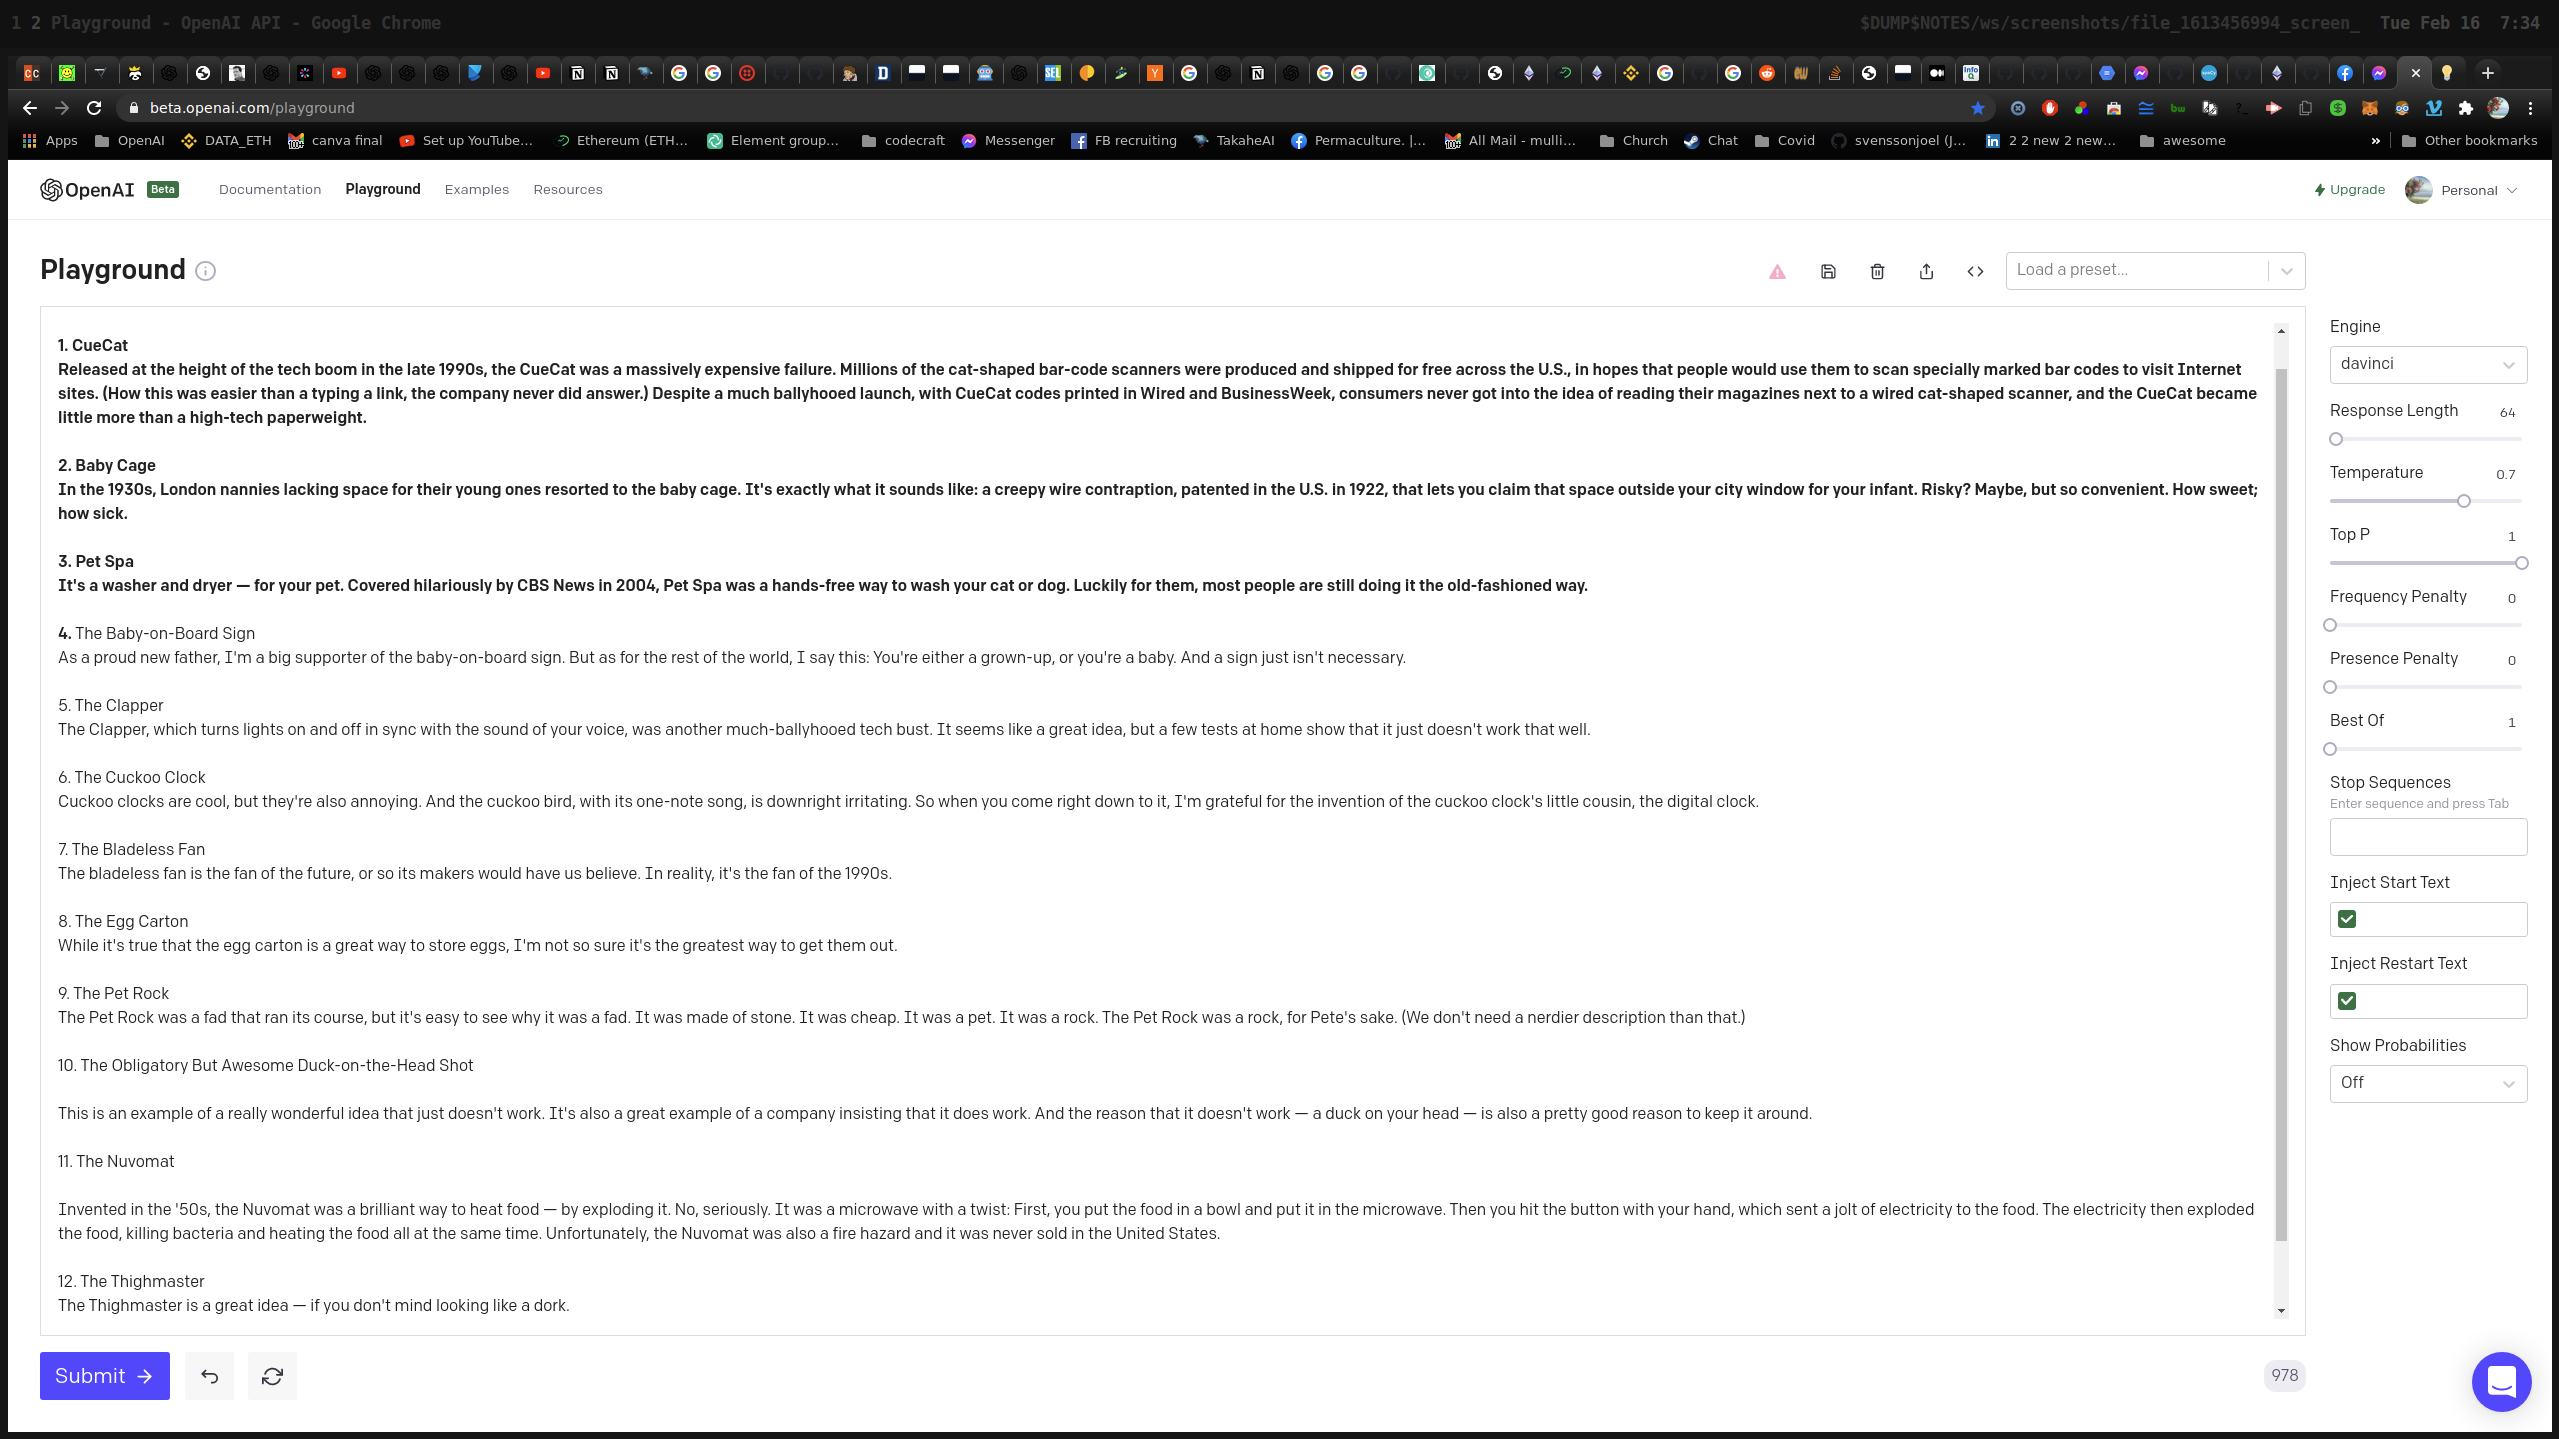
\includegraphics[width=.9\linewidth]{./silly-inventions.png}
\end{center}
\end{block}

\begin{block}{Conversation}
\begin{itemize}
\item Q\&A agent
\item Sarcastic chatbot
\end{itemize}

{\footnotesize
\url{http://github.com/semiosis/prompts/blob/master/prompts/sarcastic-response.prompt}
}
\end{block}
\end{frame}

\begin{frame}[label={sec:orgae066ea},fragile]{Design patterns}
 \begin{block}{\texttt{generate-vim-command.prompt}}
{\footnotesize
\begin{verbatim}
 1  Vim
 2  
 3  Insert "Q: " at the start of the line
 4  :%s/^/Q: /g.
 5  ###
 6  Remove whitespace from the start of each line
 7  :%s/^\s*/\1/g
 8  ###
 9  Join each line with the next line
10  :1,$j
11  ###
12  Make all occurrences of Steve lowercase
13  :%s/Steve/steve/g
14  ###
15  <1>
\end{verbatim}
}
\end{block}
\end{frame}

\section{Explanations}
\label{sec:org6083cad}
\subsection{Using \texttt{pen.el}}
\label{sec:org48e3fc2}
\begin{frame}[label={sec:orgfac0ea1},fragile]{Prompt YAML format Part 1}
 \begin{block}{\texttt{meeting-bullets-to-summary.prompt}}
\begin{verbatim}
 1  title: "meeting bullet points to summary"
 2  prompt: |+
 3      Convert my short hand into a first-hand
 4      account of the meeting:
 5  
 6      <1>
 7  
 8      Summary:
 9  engine: "davinci-instruct-beta"
10  temperature: 0.7
11  max-tokens: 60
\end{verbatim}
\end{block}
\end{frame}

\begin{frame}[label={sec:orgd24216e},fragile]{Prompt YAML format Part 2}
 \begin{block}{\texttt{meeting-bullets-to-summary.prompt}}
\begin{verbatim}
1  top-p: 1
2  frequency-penalty: 0.0
3  presence-penalty: 0.0
4  best-of: 1
5  stop-sequences:
6  - "\n\n"
7  conversation-mode: no
8  stitch-max: 0
\end{verbatim}

\begin{description}
\item[{stitch-max}] Keep stitching together until reaching this limit.
This allows a full response for answers which may need n*max-tokens to reach the stop-sequence.
\end{description}
\end{block}
\end{frame}

\begin{frame}[label={sec:orgb2c7a78},fragile]{Prompt YAML format: Part 3}
 \begin{block}{\texttt{meeting-bullets-to-summary.prompt}}
\begin{verbatim}
1  vars:
2  - "notes"
3  examples:
4  - |+
5      Tom: Profits up 50%
6      Jane: New servers are online
7      Kjel: Need more time to fix software
8      Jane: Happy to help
9      Parkman: Beta testing almost done
\end{verbatim}
\end{block}
\end{frame}

\section{\texttt{semiosis}}
\label{sec:org7812ed8}
\subsection{\texttt{pen.el}}
\label{sec:org6a0713c}
\begin{frame}[label={sec:org9d1d276},fragile]{\texttt{Prompts as functions}}
 \begin{block}{\texttt{pen-generate-prompt-functions}}
Generate prompt functions for the files in the
prompts directory Function names are prefixed
with \texttt{pen-pf-} for easy searching.

\url{http://github.com/semiosis/prompts}
\end{block}
\end{frame}

\subsection{\texttt{examplary}}
\label{sec:orgdb5ef62}
\begin{frame}[label={sec:org7157426},fragile]{\texttt{examplary}: examples as functions}
 An example-oriented DSL that can be used to
construct and compose NLP tasks.

Why is a DSL needed for this? Just to make the
code a little more terse.

\begin{block}{Regex}
\url{https://github.com/pemistahl/grex}

{\footnotesize
\begin{verbatim}
1  (def regex
2    "example 1\nexample2" "^example [12]$"
3    "example 2\nexample3" "^example [23]$"
4    "pi4\npi5" "^pi[45]$")
\end{verbatim}
}
\end{block}
\end{frame}

\begin{frame}[label={sec:org113cb93},fragile]{\texttt{examplary}: examples as functions}
 \begin{block}{Analogy}
{\footnotesize
\begin{verbatim}
 1  (def analogy
 2    ;; Each line is a training example.
 3    "NNs" "NNs are like genetic algorithms in
 4    that both are systems that learn from
 5    experience"
 6    "Social media" "Social media is like a
 7    market in that both are systems that
 8    coordinate the actions of many
 9    individuals.")
10  
11  (def field
12    "chemistry" "study of chemicals"
13    "biology" "study of living things")
\end{verbatim}
}
\end{block}
\end{frame}

\section{Demonstrations}
\label{sec:orgdef31ef}
\begin{frame}[label={sec:orgf53798a}]{Something funny}
\begin{block}{Vexate a simple instruction}
\begin{center}
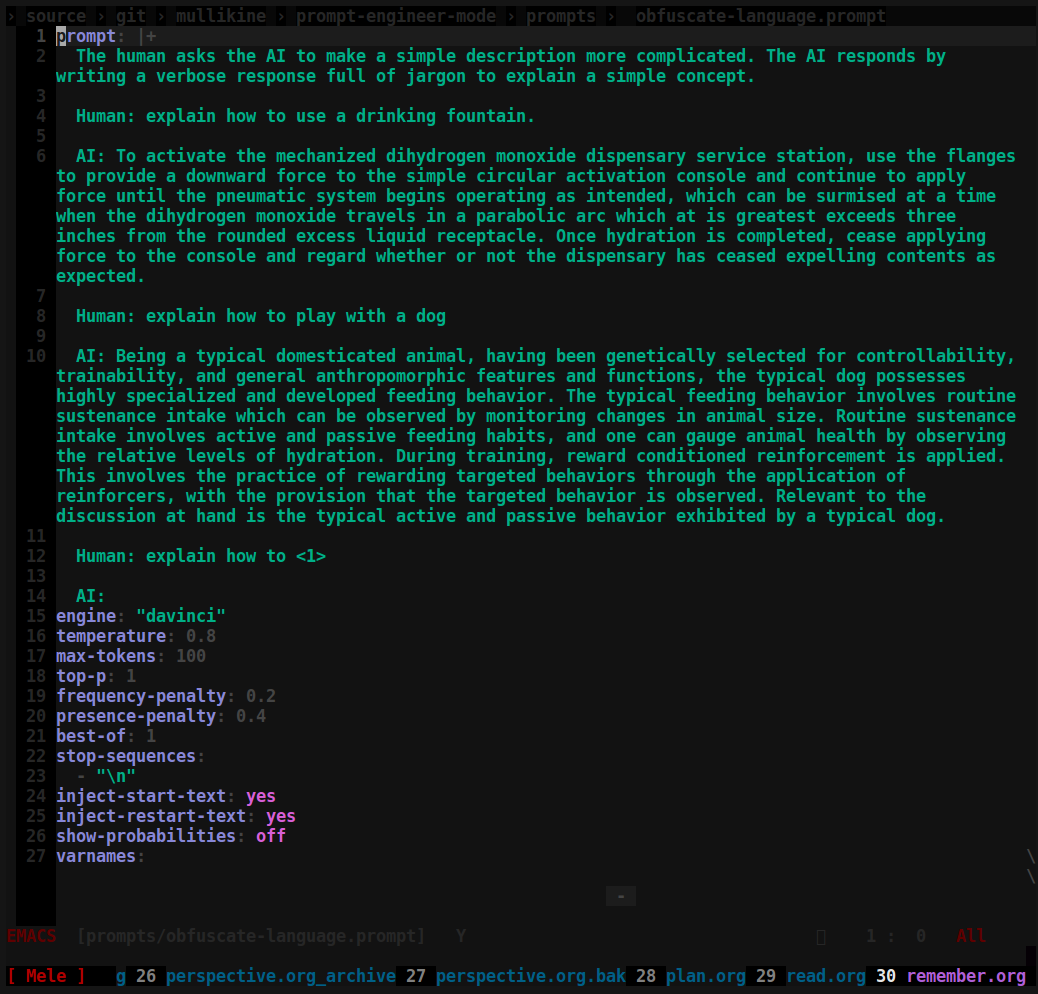
\includegraphics[width=.9\linewidth]{./complicate.png}
\end{center}
\end{block}
\end{frame}

\begin{frame}[label={sec:org9a72146}]{Something funny}
\begin{block}{How to crack an egg}
\begin{center}
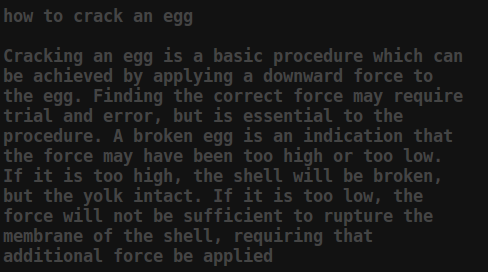
\includegraphics[width=.9\linewidth]{./crack-an-egg.png}
\end{center}
\end{block}
\end{frame}

\begin{frame}[label={sec:orgcd99f69}]{Create a prompt}
\begin{block}{Ask the audience}
\begin{itemize}
\item What type of text to generate
\begin{itemize}
\item Could be code, prose, etc.
\end{itemize}
\end{itemize}
\end{block}
\end{frame}

\section{Appendix}
\label{sec:orgde7c4dd}
\subsection{Additional reading}
\label{sec:org27f379e}
\begin{frame}[label={sec:orgc59c524}]{Tutorials}
\begin{block}{Ruby}
{\footnotesize
\url{https://www.twilio.com/blog/generating-cooking-recipes-openai-gpt3-ruby}
}
\end{block}
\end{frame}
\end{document}
